\documentclass[8pt]{extarticle}
\usepackage[a4paper,landscape,top=1.15cm,bottom=1.05cm,left=0.9cm,right=0.9cm,headsep=0.25cm,footskip=0.45cm]{geometry}
\usepackage{xeCJK}
\setCJKmainfont{Noto Serif CJK SC}[BoldFont={Noto Serif CJK SC Bold}]
\setCJKsansfont{Noto Sans CJK SC}
\setCJKmonofont{Noto Sans Mono CJK SC}
\setmonofont{DejaVu Sans Mono}[Scale=0.88]
\usepackage{amsmath,amssymb}
\usepackage[dvipsnames]{xcolor}
\usepackage{graphicx,multicol,booktabs,tabularx,array,enumitem,fancyhdr,needspace,fancyvrb,newunicodechar}
\usepackage[most]{tcolorbox}
\usepackage[hidelinks]{hyperref}

\newunicodechar{→}{\ensuremath{\rightarrow}}
\newunicodechar{←}{\ensuremath{\leftarrow}}
\newunicodechar{≥}{\ensuremath{\geq}}
\newunicodechar{≤}{\ensuremath{\leq}}
\newunicodechar{×}{\ensuremath{\times}}
\newunicodechar{≈}{\ensuremath{\approx}}
\newunicodechar{τ}{\ensuremath{\tau}}
\newunicodechar{−}{\ensuremath{-}}
\newunicodechar{⊂}{\ensuremath{\subset}}

\definecolor{cred}{HTML}{C0392B}\definecolor{cblue}{HTML}{2C3E9E}
\definecolor{cgreen}{HTML}{1E7A4C}\definecolor{cpurple}{HTML}{6C3483}
\definecolor{cteal}{HTML}{117A65}\definecolor{cgray}{HTML}{5D6D7E}
\definecolor{corange}{HTML}{B9770E}
\setlength{\columnsep}{11pt}\setlength{\columnseprule}{0.3pt}
\setlength{\parindent}{0pt}\setlength{\parskip}{1.5pt}
\linespread{1.0}
\setlist{nosep,leftmargin=1.0em,labelsep=0.3em}
\setlist[itemize]{label={\color{cgray}\textbullet}}
\newcolumntype{Y}{>{\raggedright\arraybackslash}X}
\setlength{\tabcolsep}{3pt}

\pagestyle{fancy}\fancyhf{}
\fancyhead[L]{\small LLM Agent 速查表 \#01}
\fancyhead[C]{\small\textsc{Cheatsheet: Tool Calling in LLMs}}
\fancyhead[R]{\small\texttt{2015 → 2026}}
\fancyfoot[L]{\small Prepared by Yiwen, with help from Claude}
\fancyfoot[C]{\small\thepage}\fancyfoot[R]{\small\textsc{Fall 2026}}
\renewcommand{\headrulewidth}{0.5pt}\renewcommand{\footrulewidth}{0.5pt}

\newcommand{\sect}[2][cred]{\par\vspace{4pt}{\color{#1}\rule[-2pt]{2.5pt}{10pt}}\hspace{3pt}{\large\bfseries\color{#1}#2}\par\nopagebreak\vspace{1pt}}
\newcommand{\sub}[1]{\par\vspace{2pt}{\bfseries\color{cteal}#1}\par\nopagebreak}
\newcommand{\paper}[2]{\par\vspace{3pt}{\bfseries\color{cblue}#1}\ {\scriptsize\color{cgray}#2}\par\nopagebreak}
\newcommand{\lab}[1]{{\bfseries\color{cred}#1}\,}
\newcommand{\ax}[1]{\href{https://arxiv.org/abs/#1}{\texttt{#1}}}
\newcommand{\note}[1]{\par{\itshape\color{cblue}#1}\par}

\newtcolorbox{tbox}[2][]{enhanced,colback=#2!5,colframe=#2!65,boxrule=0.5pt,arc=1.5pt,
  left=3pt,right=3pt,top=1.5pt,bottom=1.5pt,fonttitle=\bfseries\small,coltitle=black,colbacktitle=#2!16,
  toptitle=0.5pt,bottomtitle=0.5pt,before skip=3pt,after skip=3pt,#1}
\newenvironment{code}{\VerbatimEnvironment\begin{tcolorbox}[colback=gray!7,colframe=gray!45,boxrule=0.4pt,arc=1pt,left=2pt,right=2pt,top=0.5pt,bottom=0.5pt,before skip=2pt,after skip=2pt]\begin{Verbatim}[fontsize=\scriptsize]}{\end{Verbatim}\end{tcolorbox}}

\begin{document}
%==================== HEADER ====================
\begin{tcolorbox}[enhanced,colback=cblue!5,colframe=cblue!40,boxrule=0.6pt,arc=2pt,left=7pt,right=7pt,top=4pt,bottom=4pt]
\begin{minipage}[t]{0.56\linewidth}
{\fontsize{17}{21}\selectfont\bfseries Cheatsheet: 大模型 Tool Calling（2015 → 2026）}\par\vspace{2pt}
{\itshape\color{cgray} Mechanisms · Objectives · Formats · Numbers — from retrieval to agentic RL}\par
{\small\color{cgray} Yiwen 整理 · 70+ 篇论文与官方发布 · 数字均出自原文（arXiv v1 / 官方博客）· 2026 年 10 月核对}
\end{minipage}\hfill
\begin{minipage}[t]{0.42\linewidth}\small
\textbf{怎么读：}每节按 \textbf{\color{cred}问题} → \textbf{\color{cblue}方法（机制 / 公式 / 格式）} → \textbf{数字} → \textbf{\color{corange}局限} 组织。
\textbf{记号：}$x$ 输入，$a_t$ 动作，$o_t$ 工具返回（观察），$y$ 最终答案，$\pi_\theta$ 策略模型，$r$ 奖励，$\tau$ 轨迹。
所有 arXiv 编号可点击。
\end{minipage}
\end{tcolorbox}

\begin{minipage}[t]{0.37\linewidth}\vspace{0pt}
\begin{tbox}[title={统一形式化：tool use = 部分可观测的序列决策}]{cblue}
\small
\textbf{轨迹}\ \ $\tau=(x,\,a_1,o_1,\,\dots,\,a_T,o_T,\,y)$，\ $a_t\in\mathcal{L}\cup\mathcal{T}$\\
$\mathcal{L}$：自由文本（思考），不改变环境；$\mathcal{T}$：工具调用，$o_t=\mathrm{Env}(a_t)$\\
\textbf{策略}\ \ $a_t\sim\pi_\theta(\cdot\mid x,a_{<t},o_{<t})$\\[2pt]
\textbf{四类学习信号}
\begin{enumerate}
\item 提示（不训练）：few-shot 轨迹示范（ReAct、MRKL）
\item 模仿 / SFT：$\mathcal{L}=-\sum_t m_t\log\pi_\theta(a_t\mid h_t)$，\\$m_t=0$ 屏蔽工具返回 token（只学“怎么调”，不学“预测结果”）
\item 自监督过滤：保留\textbf{降低后文 LM 损失}的调用（Toolformer）
\item 结果奖励 RL：$\max_\theta\ \mathbb{E}_{\tau\sim\pi_\theta}[\,r(x,y)\,]-\beta\,\mathrm{KL}(\pi_\theta\Vert\pi_{\mathrm{ref}})$
\end{enumerate}
\textbf{三个子问题}：\ \textbf{何时}调（触发）· \textbf{调什么}（选择 + 填参）· \textbf{怎么用}返回值（整合 / 纠错）
\end{tbox}
\end{minipage}\hfill
\begin{minipage}[t]{0.615\linewidth}\vspace{0pt}
\begin{tbox}[title={范式对照：每一代由谁决定调用、靠什么学会}]{cgreen}
\small
\begin{tabularx}{\linewidth}{@{}p{1.55cm} p{2.6cm} p{3.4cm} Y@{}}
\toprule
范式 & 代表 & 调用决策 / 学习信号 & 带来的新问题\\\midrule
{\color{cblue}固定检索} & REALM、RAG & 每次输入都检索；端到端边缘化 & 不能按需、只查一次\\
{\color{cblue}人类示范} & WebGPT、LaMDA & BC + 奖励模型 + best-of-$n$ & 标注贵，单工具\\
{\color{cblue}提示 / 路由} & MRKL、ReAct、Self-Ask & few-shot 轨迹，模型在上下文中决定 & 依赖提示，长轨迹易循环\\
{\color{cblue}自监督} & Toolformer、TALM & 损失下降过滤 / self-play 自举 & 不能链式调用，工具少\\
{\color{cblue}大规模 SFT} & Gorilla、ToolLLM & 合成指令 + 搜索得到的解路径 & 参数幻觉、需检索工具\\
{\color{cblue}标准接口} & Function calling、MCP & JSON Schema / JSON-RPC 协议 & 工具定义撑爆上下文\\
{\color{cblue}代码即行动} & PAL、CodeAct、SWE-agent & 生成可执行代码组合调用 & 沙箱与执行安全\\
{\color{cred}结果奖励 RL} & Search-R1、ReTool、ToolRL & 只看最终答案对错 + 格式 & 奖励设计、长程信用分配\\
\bottomrule
\end{tabularx}
\end{tbox}
\end{minipage}

\vspace{1pt}
\begin{multicols}{4}
%==================== 0 ====================
\sect{0. 前史：检索是第一个“工具”（2015–2020）}
\begin{tbox}[title=问题]{cred}\small
参数化知识有截止日期、难更新、无法溯源；扩大模型容量代价高。
\end{tbox}
\paper{Neural Module Networks}{Berkeley · \ax{1511.02799} · 2015-11}
按问题的句法解析，动态拼装 \texttt{find} / \texttt{describe} 等小神经模块做 VQA。“按问题组合模块”的思想先于 LLM。
\paper{REALM}{Google · \ax{2002.08909} · 2020-02}
\begin{itemize}
\item $p(y|x)=\sum_z p(y|z,x)\,p(z|x)$\\ $p(z|x)\propto\exp\big(\mathrm{Emb}_{\text{in}}(x)^{\top}\mathrm{Emb}_{\text{doc}}(z)\big)$
\item 检索器参与 MLM \textbf{预训练}，梯度回传到检索器；文档索引（MIPS）异步刷新。
\end{itemize}
\paper{RAG}{FAIR / UCL / NYU · \ax{2005.11401} · 2020-05}
\begin{itemize}
\item 检索器 DPR（BERT 双塔）+ 生成器 BART，对 top-$k$ 文档边缘化：
\item \textbf{RAG-Seq}（整段答案共用一篇文档）：\\ $p(y|x)\approx\sum_{z}p_\eta(z|x)\prod_i p_\theta(y_i|x,z,y_{<i})$
\item \textbf{RAG-Tok}（每个 token 可换文档）：\\ $p(y|x)\approx\prod_i\sum_{z}p_\eta(z|x)\,p_\theta(y_i|x,z,y_{<i})$
\item 文档编码器冻结（免重建索引），只训查询编码器和生成器。
\end{itemize}
\begin{tbox}[title=局限]{corange}\small
检索是\textbf{写死}的：每个输入检索一次，模型不决定“要不要查、查什么、查几次”。
\end{tbox}

%==================== 1 ====================
\sect{1. 学会多步操作一个工具（2021–2022）}
\paper{WebGPT}{OpenAI · \ax{2112.09332} · 2021-12}
\lab{环境}纯文本浏览器（Bing 搜索）。\lab{动作}
\begin{code}
Search <query>      Clicked on link <id>
Find in page <text> Quote: <text>
Scrolled down/up <1,2,3>    Top   Back
End: Answer   End: <Nonsense, Controversial>
\end{code}
\begin{itemize}
\item 回答只能基于收集到的 \textbf{Quote} → 自带引用，便于人工核查事实。
\item \textbf{四种训练}：行为克隆 BC · 奖励模型 RM（人类成对比较）· RL（PPO + KL）· 拒绝采样 best-of-$n$（$n$=4/16/64）。
\item 最优：175B BC + \textbf{best-of-64}（按 RM 选）；RL 增益小于拒绝采样。
\item ELI5：\textbf{56\%} 胜人类示范者，\textbf{69\%} 胜 Reddit 最高赞。模型 760M / 13B / 175B。
\end{itemize}
\paper{LaMDA}{Google · \ax{2201.08239} · 2022-01}
工具集 TS =\{信息检索, 计算器, 翻译器\}。模型先生成发给 TS 的查询，结果拼回上下文再生成回答；用众包标注的“何时查、查什么”数据微调。
\paper{Lazaridou et al.}{DeepMind · \ax{2203.05115} · 2022-03}
不微调：Google 搜索 → 切段落 → few-shot 提示条件生成；多段落各生成候选答案，再用模型概率重排。
\begin{tbox}[title=局限]{corange}\small
需要大量人类示范 / 标注；一个模型只会一个工具。
\end{tbox}

%==================== 2 ====================
\sect{2. 大模型当路由器 · 自举（2022）}
\paper{MRKL}{AI21 Labs · \ax{2205.00445} · 2022-05}
\begin{itemize}
\item 架构：LLM \textbf{router} + 可插拔专家模块（神经：其他模型；符号：计算器、货币换算、数据库、天气 API）。
\item 主张：符号模块可解释、可更新，不需重训大模型。
\item 关键难点是\textbf{参数抽取}：在 Jurassic-X 上用合成数据训练从自然语言抽取算术参数，测试跨位数、跨运算、跨问法的泛化。
\end{itemize}
\paper{TALM}{Google · \ax{2205.12255} · 2022-05}
\begin{code}
input |tool-call  tool args |result  tool output
      |output  final answer
\end{code}
\lab{自举}从少量示范出发：采样工具输入 → 调用 → 若最终输出与目标匹配就加入训练集 → 再微调，迭代（iterative self-play）。任务：NQ（检索）、MathQA（求解器）。

%==================== 3 ====================
\sect{3. 代码就是工具（2022）}
\paper{PAL}{CMU · \ax{2211.10435} · 2022-11}
LM 只把题目“翻译”成 Python（变量名 + 注释即推理），解释器求值：
\begin{code}
# Roger has 5 balls. He buys 2 cans,
# each has 3 balls.
tennis_balls = 5
bought_balls = 2 * 3
answer = tennis_balls + bought_balls
\end{code}
\begin{itemize}
\item Codex：GSM8K \textbf{72.0}，比 PaLM-540B + CoT 高 \textbf{15} 个点（绝对）。
\item 把题中数字换成大数（GSM-Hard）后 CoT 明显下降、PAL 受影响小 → 错误主要来自\textbf{计算}而不是理解。
\end{itemize}
\paper{Program of Thoughts}{Waterloo · \ax{2211.12588} · 2022-11}
同一思路扩展到数值 / 金融 QA（FinQA、TAT-QA 等），平均比 CoT 高约 \textbf{12\%}。
\note{要点：把“计算”从 LM 中拆出去；代码解释器此后成为最通用的工具。}

%==================== 4 ====================
\sect{4. 推理与行动交替（2022）}
\paper{ReAct}{Princeton / Google · \ax{2210.03629} · 2022-10}
\begin{itemize}
\item 增广动作空间 $\hat{\mathcal{A}}=\mathcal{A}\cup\mathcal{L}$：thought 不影响环境，只更新上下文。
\item Wikipedia API：\texttt{search[entity]} · \texttt{lookup[string]} · \texttt{finish[answer]}
\item 只用 few-shot 人写轨迹提示 PaLM-540B，不训练。
\item 知识任务：thought 与 action 密集交替；决策任务：thought 稀疏，由模型自己决定何时想。
\end{itemize}
\begin{code}
Thought 1: 需要先找到 X 的出生地
Action 1:  search[X]
Obs 1:     X ... was born in Lyon ...
Thought 2: 再查里昂人口
Action 2:  lookup[population] ...
\end{code}
{\small
\begin{tabularx}{\linewidth}{@{}Y r r@{}}
\toprule
PaLM-540B & HotpotQA EM & FEVER Acc\\\midrule
Standard & 28.7 & 57.1\\
CoT & 29.4 & 56.3\\
CoT-SC & 33.4 & 60.4\\
Act（无 thought） & 25.7 & 58.9\\
ReAct & 27.4 & 60.9\\
CoT-SC → ReAct & 34.2 & \textbf{64.6}\\
ReAct → CoT-SC & \textbf{35.1} & 62.0\\
\bottomrule
\end{tabularx}}
\begin{itemize}
\item 决策：ALFWorld 成功率 ReAct \textbf{71} vs Act 45 vs BUTLER 37（多个提示取最好；ReAct 平均 57）；WebShop ReAct 40.0 vs 模仿学习 29.1。
\item 失败分析：CoT 失败中 \textbf{56\%} 是幻觉；ReAct 主要失败是推理错误 / 重复循环（47\%）和搜索没有返回有用信息（23\%）。
\item 组合规则：ReAct 在步数内没给出答案 → 回退 CoT-SC；CoT-SC 多数票不足 $n/2$ → 回退 ReAct。内部知识与外部检索\textbf{互补}。
\end{itemize}
\paper{Self-Ask}{UW / MosaicML 等 · \ax{2210.03350} · 2022-10}
\lab{组合性差距}模型答对两个子问题却答错组合问题的比例；在 GPT-3 系列中不随规模缩小。
\begin{code}
Are follow up questions needed here: Yes.
Follow up: <子问题>      ← 可直接交给搜索引擎
Intermediate answer: <答案>
So the final answer is: <答案>
\end{code}
\paper{IRCoT}{Stony Brook / Allen AI · \ax{2212.10509} · 2022-12}
\begin{code}
D ← Retrieve(q); cot ← ""
loop:
  s ← LM_next_sentence(q, D, cot)
  cot += s; D ∪= Retrieve(s)   # 用最新一句当查询
until "answer is" in s or 步数上限
\end{code}
HotpotQA / 2Wiki / MuSiQue / IIRC：检索最多 +21 个点，QA 最多 +15 个点。
\note{要点：工具调用从此嵌在推理轨迹\emph{里面}，每一步观察都影响下一步。}

%==================== 5 ====================
\sect{5. 自监督学会“何时调用”（2023）}
\paper{Toolformer}{Meta · \ax{2302.04761} · 2023-02}
\lab{格式}调用直接写进文本：
\begin{code}
Out of 1400 participants, 400 (or
[Calculator(400 / 1400) → 0.29] 29%)
passed the test.
\end{code}
\lab{流程}
\begin{enumerate}
\item \textbf{采样位置}：$p_i=p_M(\texttt{<API>}\mid P(x),x_{1:i-1})$，保留 $p_i>\tau_s$ 的前 $k$ 个位置，每处采样 $m$ 个调用 $c_i$（默认 $\tau_s$=0.05, $k$=5, $m$=5）。
\item \textbf{执行}得到结果 $r_i$。
\item \textbf{过滤}：加权损失\\
$L_i(z)=-\sum_{j=i}^{n}w_{j-i}\log p_M(x_j\mid z,x_{1:j-1})$，\\
$\tilde w_t=\max(0,1-0.2t)$（归一化）\\
$L_i^+=L_i(e(c_i,r_i))$\\
$L_i^-=\min\big(L_i(\varepsilon),\,L_i(e(c_i,\varepsilon))\big)$\\
保留 $L_i^- - L_i^+\ge\tau_f$（默认 1.0）：\textbf{“调用+结果”比“不调”和“调了不给结果”都更能帮助预测后文}。
\item \textbf{微调}：在增广语料上用普通 LM 目标（原文本不变 → 不损语言能力）。
\item \textbf{推理}：正常解码，遇到 “→” 暂停，执行调用，插入结果和 “]” 后继续。
\end{enumerate}
\begin{itemize}
\item 工具：QA（Atlas）、Wikipedia 搜索、计算器、日历、机器翻译；基座 GPT-J 6.7B。
\item 零样本数学、QA 等任务上常胜过大得多的模型（如 GPT-3 175B），且困惑度不变差。
\end{itemize}
\begin{tbox}[title=局限]{corange}\small
每个调用独立生成 → \textbf{不能链式}使用工具；不能交互（如改写查询、浏览）；对计算器等工具样本效率低。
\end{tbox}

%==================== 6 ====================
\sect{6. LLM 当总指挥：调用其他模型（2023）}
\paper{HuggingGPT}{浙大 / MSRA · \ax{2303.17580} · 2023-03}
四阶段：\textbf{任务规划 → 模型选择 → 任务执行 → 回答生成}。
\begin{code}
[{"task": "image-to-text", "id": 0, "dep": [-1],
  "args": {"image": "a.jpg"}},
 {"task": "text-to-speech", "id": 1, "dep": [0],
  "args": {"text": "<resource>-0"}}]
\end{code}
模型选择：按任务类型过滤 Hugging Face 模型，按下载量取前 $K$ 个，把模型描述放进上下文让 LLM 选。\texttt{<resource>-id} 表示依赖前一任务的输出。
\paper{ViperGPT}{Columbia · \ax{2303.08128} · 2023-03}
给 Codex 一个视觉 API 规格（\texttt{ImagePatch.find / exists / verify\_property / simple\_query} 等），让它写 Python 程序回答视觉问题；零样本、无需训练。
\paper{Chameleon}{UCLA / MSR · \ax{2304.09842} · 2023-04}
LLM 规划器输出\textbf{模块序列}（知识检索、Bing 搜索、图像描述、OCR、程序生成 / 验证 / 执行、表格查找、答案生成），按序执行。GPT-4：ScienceQA \textbf{86.54\%}，TabMWP \textbf{98.78\%}。
\paper{Visual ChatGPT}{MSRA · \ax{2303.04671} · 2023-03}
Prompt Manager 把多个视觉基础模型的输入输出转成文本，ChatGPT 多轮调度做图像编辑 / 生成。

%==================== 7 ====================
\sect{7. 扩到上千、上万个 API（2023）}
\begin{tbox}[title=问题]{cred}\small
工具从个位数涨到上万：\textbf{选对}哪个 API、\textbf{填对}参数、不\textbf{编造}不存在的 API。
\end{tbox}
\paper{API-Bank}{阿里达摩院 · \ax{2304.08244} · 2023-04}
可运行评测：73 个 API、314 段对话、753 次调用。三个能力层级：\textbf{Call}（给定 API）→ \textbf{Retrieve+Call}（先检索）→ \textbf{Plan+Retrieve+Call}（多步规划）。
\paper{Gorilla}{Berkeley · \ax{2305.15334} · 2023-05}
\begin{itemize}
\item APIBench：TorchHub 94 + TensorHub 626 + HuggingFace 925 = \textbf{1,645} 个 API（筛选后）；self-instruct 生成“指令–API”对，微调 LLaMA-7B。
\item \textbf{Retriever-aware training}：训练时在指令后附检索到的文档：
\end{itemize}
\begin{code}
<instruction> Use this API documentation for
reference: <retrieved_API_doc_JSON>
\end{code}
\begin{itemize}
\item 评测用 \textbf{AST 子树匹配}；\textbf{幻觉} = 生成的 API 不在库中，\textbf{错误} = 在库中但不对。
\item 发现：检索器质量差时，带检索反而可能比零检索差 → 检索质量是瓶颈。
\end{itemize}
\paper{ToolLLM / ToolBench}{清华 · \ax{2307.16789} · 2023-07}
\begin{enumerate}
\item \textbf{收集}：RapidAPI 上 3,451 个工具、\textbf{16,464} 个 API、49 类。
\item \textbf{造指令}：采样 API → ChatGPT 写指令；I1 单工具 / I2 同类多工具 / I3 同集合多工具。
\item \textbf{标解路径}：ChatGPT function calling + \textbf{DFSDT}。
\end{enumerate}
\lab{DFSDT}深度优先决策树：每个节点是一次调用后的状态；扩展子节点时把已有兄弟节点告诉模型，以生成\textbf{不同}的动作；失败或放弃就\textbf{回溯}；找到一条有效路径即停。比 ReAct 单链在 I2 / I3 上解决率高很多。\\
\lab{ToolEval}\textbf{pass rate}（在限定预算内完成）+ \textbf{win rate}（与 ChatGPT-ReAct 对比，ChatGPT 当评委）。\\
\lab{模型}ToolLLaMA（LLaMA-2 7B）+ API 检索器，在未见过的 API 上也能泛化，接近 ChatGPT。

%==================== 8 ====================
\sect{8. 产品化与标准接口（2023–2025）}
\paper{Function calling}{OpenAI · 2023-06}
\begin{code}
→ tools=[{"type":"function","function":{
    "name":"get_weather",
    "description":"Get current weather",
    "parameters":{"type":"object",
      "properties":{"city":{"type":"string"}},
      "required":["city"]}}}]
← assistant.tool_calls=[{"id":"call_1",
    "function":{"name":"get_weather",
    "arguments":"{\"city\":\"Chicago\"}"}}]
→ {"role":"tool","tool_call_id":"call_1",
   "content":"12°C, cloudy"}
← assistant: 芝加哥现在 12°C，多云。
\end{code}
\begin{itemize}
\item 模型\textbf{只产出调用}，由应用执行；\texttt{arguments} 是 JSON 字符串，需要校验。
\item \texttt{tool\_choice}：auto / none / required / 指定函数。并行调用（2023-11）；\texttt{strict} 模式保证符合 Schema（Structured Outputs，2024-08）。
\item 训练侧：工具描述放在系统区，模型经 SFT/RLHF 学会输出结构化调用——“何时调用”交给模型，“如何执行”交给应用。
\end{itemize}
\paper{Model Context Protocol}{Anthropic · 2024-11 · 规范见 modelcontextprotocol.io}
{\small
\begin{tabularx}{\linewidth}{@{}l Y@{}}
\toprule
组件 & 说明\\\midrule
架构 & Host（应用）内含多个 Client，每个 Client 1:1 连一个 Server\\
消息 & JSON-RPC 2.0\\
Server 原语 & \textbf{Tools}（模型控制）· \textbf{Resources}（应用控制）· \textbf{Prompts}（用户控制）\\
Client 原语 & \textbf{Sampling}（Server 请求 LLM 补全）· \textbf{Roots} · \textbf{Elicitation}（向用户要输入）\\
传输 & stdio（本地）· Streamable HTTP（远程，2025-03 取代 HTTP+SSE）\\
授权 & OAuth 2.1（2025-03 起）\\
\bottomrule
\end{tabularx}}
\begin{code}
{"jsonrpc":"2.0","id":7,"method":"tools/call",
 "params":{"name":"get_weather",
           "arguments":{"city":"Chicago"}}}
← {"result":{"content":[{"type":"text",
   "text":"12°C, cloudy"}],"isError":false}}
\end{code}
\note{价值：$M$ 个应用 × $N$ 个工具的集成问题 → $M+N$。}

%==================== 9 ====================
\sect{9. 用工具和反馈检查自己（2023）}
\paper{Reflexion}{Northeastern / MIT / Princeton · \ax{2303.11366} · 2023-03}
\begin{itemize}
\item 三个角色：Actor $M_a$（生成轨迹）、Evaluator $M_e$（打分：单元测试 / 规则 / LLM）、Self-Reflection $M_{sr}$（把失败写成文字反思）。
\item 反思存入情景记忆（只保留最近 1–3 条），下一次尝试拼进上下文。\textbf{“verbal RL”}：不更新权重，反思文本充当“语义梯度”。
\item HumanEval pass@1 \textbf{91\%}（GPT-4 为 80.1\%）；AlfWorld 134 个任务完成 130 个（+22\%）；HotpotQA +20\%。
\end{itemize}
\paper{CRITIC}{清华 / MSRA · \ax{2305.11738} · 2023-05}
$y_0\to$ 用工具验证得到评语 $c_i\to y_{i+1}=\mathrm{LM}(x,y_i,c_i)$，迭代。工具：搜索（事实 QA）、代码解释器（数学）、Perspective API（毒性）。\textbf{去掉工具只靠自我批评，提升很小甚至下降}——外部反馈是关键。
\paper{LATS}{UIUC · \ax{2310.04406} · 2023-10}
把 ReAct 放进 \textbf{MCTS}：选择 → 扩展（采样 $n$ 个动作）→ 评估 → 模拟 → 回传 → 反思。
\begin{itemize}
\item $\mathrm{UCT}(s)=V(s)+w\sqrt{\ln N(p)/N(s)}$
\item $V(s)=\lambda\cdot$LM 打分 $+(1-\lambda)\cdot$自一致性分数
\item HumanEval \textbf{92.7\%}（GPT-4）；WebShop 平均分 75.9（GPT-3.5）。
\item 代价：需要\textbf{可回退}的环境，调用次数大幅增加。
\end{itemize}

%==================== 10 ====================
\sect{10. 自己造工具、积累技能（2023）}
\paper{LATM}{Princeton / Google · \ax{2305.17126} · 2023-05}
\textbf{Tool maker}（GPT-4）：提出通用 Python 函数 → 用验证样例做\textbf{单元测试} → 封装成“函数 + 调用示例”；\textbf{Tool user}（GPT-3.5）反复调用；\textbf{dispatcher} 判断新任务是否已有缓存工具。造一次、用多次 → 降成本。
\paper{CREATOR}{清华 · \ax{2305.14318} · 2023-05}
创建 → 决策 → 执行 → \textbf{纠正}（根据报错修改工具）。把“抽象推理（造工具）”与“具体推理（用工具）”分开。
\paper{Voyager}{NVIDIA / Caltech 等 · \ax{2305.16291} · 2023-05}
\begin{itemize}
\item \textbf{自动课程}：GPT-4 根据当前状态提出下一个任务。
\item \textbf{技能库}：key = 技能描述的嵌入，value = 可执行 JS 代码；新任务检索相关技能组合使用。
\item \textbf{迭代提示}：环境反馈 + 执行报错 + 自我验证（GPT-4 判断任务是否完成），直到成功再存入技能库。
\item 对比基线：独特物品 \textbf{3.3×}，移动距离 2.3×，科技树里程碑最快 \textbf{15.3×}。
\end{itemize}
\note{要点：能力以\emph{代码}形式随时间积累——“自我进化” agent 的雏形，也是后来 Agent Skills 的思想来源之一。}

%==================== 11 ====================
\sect{11. 代码即行动 · 为 agent 设计接口（2024）}
\paper{CodeAct}{UIUC · \ax{2402.01030} · 2024-02}
\begin{code}
# JSON 行动：每个调用一轮
{"tool":"price","args":{"item":"A"}}
{"tool":"price","args":{"item":"B"}} ...
# Code 行动：一轮完成，含控制流和数据流
p = {i: price(i) for i in ["A","B","C"]}
best = min(p, key=p.get)
\end{code}
\begin{itemize}
\item 优势：循环 / 条件 / 变量天然组合多个工具；直接用现有 Python 库；报错信息就是反馈。
\item 17 个 LLM 上比 JSON / 文本行动成功率最多高 \textbf{20\%}，所需动作最多少 30\%（M\textsuperscript{3}ToolEval）。
\item CodeActInstruct（约 7k 条多轮轨迹）→ 微调 CodeActAgent。
\end{itemize}
\paper{SWE-agent}{Princeton · \ax{2405.15793} · 2024-05}
\lab{ACI}agent-computer interface：像为人设计 UI 一样为 LM 设计工具。
\begin{itemize}
\item 命令：\texttt{open / goto / scroll\_up / scroll\_down / search\_file / search\_dir / find\_file / edit}
\item 文件查看器每次显示 100 行；搜索结果有上限；\texttt{edit} 带\textbf{语法检查}，有语法错误就拒绝并报错。
\item 原则：动作简单、合并常用操作、反馈简洁有信息、加护栏防止连锁错误。
\item SWE-bench pass@1 \textbf{12.5\%}、Lite 18.0\%（GPT-4 Turbo），明显高于只给 shell 的基线。
\end{itemize}
\note{重心从“模型怎么调”转向“工具该怎么为模型设计”。}

%==================== 12 ====================
\sect[cteal]{12. 评测：怎么衡量会不会用工具}
{\small
\begin{tabularx}{\linewidth}{@{}p{1.45cm} Y@{}}
\toprule
基准 & 设定 · 指标 · 关键数字\\\midrule
BFCL\newline 2024-02 & AST 匹配 + 实际执行；简单 / 多选 / 并行 / 并行多选 + \textbf{无关检测}（不该调时不调）；后续版本加入多轮、agentic\\
WebArena\newline 2023-07 & 812 个任务，自建电商、论坛、GitLab、CMS 网站；GPT-4 \textbf{14.41\%} vs 人类 78.24\%\\
AgentBench\newline 2023-08 & 8 个环境：OS、数据库、知识图谱、卡牌、谜题、家务、购物、网页\\
GAIA\newline 2023-11 & 466 题、3 个难度级；人类 \textbf{92\%} vs GPT-4 + 插件 15\%\\
OSWorld\newline 2024-04 & 369 个真实桌面任务，执行脚本判定\\
τ-bench\newline 2024-06 & 零售 115 题、航空 50 题；工具 + LLM 模拟用户 + 业务规则；最终数据库状态判定\\
\bottomrule
\end{tabularx}}
\lab{pass\^{}k}（τ-bench）$k$ 次独立尝试\textbf{全部}成功的概率：
$$\text{pass}^k=\mathbb{E}_{\text{task}}\!\left[\binom{c}{k}\Big/\binom{n}{k}\right]$$
$n$ 次试验中成功 $c$ 次。与 pass@$k$（至少一次成功）相反，衡量\textbf{稳定性}。gpt-4o 完成不到 50\%，零售 pass\^{}8 不到 25\%。

%==================== 13 ====================
\sect{13. 工具 = 新攻击面（2023–2024）}
\begin{tbox}[title=威胁模型]{cred}\small
\textbf{间接提示注入}：攻击者不碰用户输入，而是把指令藏进 agent 会读到的内容（网页、邮件、文件、工具返回）。\\
\textbf{致命三要素}（Simon Willison，2025-06-16）：私有数据 + 不可信内容 + 对外通信，三者同时具备即可被窃取数据。
\end{tbox}
\paper{Indirect Prompt Injection}{Saarland / CISPA · \ax{2302.12173} · 2023-02}
在 Bing Chat 等真实应用上演示；注入途径：被动（检索到）、主动（发邮件）、用户诱导、隐藏编码。危害：信息窃取、欺诈、入侵、传播恶意内容、操纵输出、拒绝服务。
\paper{InjecAgent}{UIUC · \ax{2403.02691} · 2024-03}
1,054 个用例（17 个用户工具 × 62 个攻击者工具）；攻击类型：直接伤害、数据窃取。ReAct 提示的 GPT-4 \textbf{24\%} 被攻破；加“hacking prompt”后接近翻倍。
\paper{AgentDojo}{ETH · \ax{2406.13352} · 2024-06}
97 个任务（workspace 40 / slack 21 / travel 20 / banking 16）、629 个安全用例。指标：良性效用、受攻击时效用、攻击成功率。

%==================== 14 ====================
\sect{14. 2025–2026：训练出来的工具使用}
\sub{14a. 结果奖励 RL（agentic RL）：通用配方}
\begin{tbox}[title={Rollout · Loss mask · Reward · 优势估计}]{cblue}\small
\textbf{Rollout}：生成到 \texttt{</search>} 或 \texttt{</code>} 时暂停 → 执行 → 结果包进 \texttt{<information>} / \texttt{<interpreter>} 拼回 → 继续生成。\\
\textbf{Loss mask}：工具返回的 token \textbf{不计梯度}（否则模型去“预测检索结果”，训练不稳）。\\
\textbf{Reward}：规则化\textbf{结果奖励}（EM / F1 / 数学等价）+ 格式奖励，通常不用过程奖励模型。\\
\textbf{GRPO}：同一问题采样 $G$ 条，$\hat A_i=\dfrac{r_i-\mathrm{mean}(r_{1..G})}{\mathrm{std}(r_{1..G})}$，省去价值网络；也常用 PPO。\\
\textbf{常见涌现}：调用次数随训练上升；学会改写查询、看到报错后自己修代码。
\end{tbox}
\begin{code}
<think> 需要先确认 X 的出生年份 </think>
<search> X birth year </search>
<information> ...检索结果（mask）... </information>
<think> ... </think>
<answer> 1987 </answer>
\end{code}
{\small
\begin{tabularx}{\linewidth}{@{}l l Y@{}}
\toprule
方法 & 工具 & 奖励 / 关键设计\\\midrule
R1-Searcher & 搜索 & 两阶段：先奖励“会调检索 + 格式”，再奖励答案 F1；Reinforce++\\
Search-R1 & 搜索 & EM；检索 token 掩码；PPO / GRPO；比 RAG 基线 +41\%（7B）/ +20\%（3B）\\
ToRL & 代码 & 从 base 直接 RL（无 SFT）；7B AIME24 43.3\%\\
ReTool & 代码 & 冷启动 SFT → PPO，对 / 错 = $\pm1$；32B 训 400 步 AIME 67\%（纯文本 RL 40\%）\\
ToolRL & 函数调用 & $R_{\text{fmt}}\in\{0,1\}$ + $R_{\text{corr}}\in[-3,3]$（工具名、参数名、参数值分别匹配）；GRPO，无 KL\\
ARPO & 搜索+代码 & 工具返回后 token 熵升高 → 在高熵步\textbf{分支采样}；约一半调用量达到基线\\
\bottomrule
\end{tabularx}}
{\scriptsize\color{cgray}出处：R1-Searcher \ax{2503.05592} · Search-R1 \ax{2503.09516} · ToRL \ax{2503.23383} · ReTool \ax{2504.11536} · ToolRL \ax{2504.13958} · ARPO \ax{2507.19849} · 综述 \ax{2509.02547} · ToolVerse \ax{2607.15660}（从数百个真实 MCP 服务器自动建 RL 环境）}\par

\sub{14b. 推理中调用工具}
\begin{itemize}
\item \textbf{OpenAI deep research}（2025-02）：o3 在浏览 + Python 任务上端到端 RL。
\item \textbf{o3 / o4-mini}（2025-04）：在思维链内组合调用全部 ChatGPT 工具。
\item \textbf{Claude 4}（2025-05）：工具调用之间可继续思考（interleaved thinking）。
\item \textbf{通义 DeepResearch}（\ax{2510.24701}）：开源 30.5B MoE（激活 3.3B），agentic 继续预训练 + SFT + RL。
\item \textbf{DeepSeek-V3.2}（\ax{2512.02556}）：思考融入工具使用；合成 1,800+ 环境、85,000 条复杂提示的 agent 训练数据。
\end{itemize}

\sub{14c. 接口标准化}
A2A（Google，2025-04；2025-06 移交 Linux 基金会）· OpenAI 支持远程 MCP（2025-05）· Agent Skills（Anthropic，2025-10；2025-12 开放标准）· Agentic AI Foundation（2025-12，MCP 移交 Linux 基金会）· MCP Apps（2026-01，工具可返回交互界面）· MCP 2026-07-28 规范（无状态，去掉 session 与 initialize 握手）。

\sub{14d. 上下文成为瓶颈：context engineering}
\begin{tbox}[title=问题]{cred}\small
几十个 MCP 服务器的工具定义 + 中间结果全部进上下文 → 贵、慢、选错工具。
\end{tbox}
\begin{itemize}
\item \textbf{Tool search}：工具定义标记延迟加载（\texttt{defer\_loading}），模型先搜索再加载需要的（Anthropic 2025-11；GPT-5.4 2026-03：36 个 MCP 服务器上 token 减少 47\%，准确率不变）。
\item \textbf{Programmatic tool calling / Code execution with MCP}（2025-11）：把工具暴露成代码 API，模型写代码调用，中间结果留在沙箱、只返回需要的部分；示例 150k → 2k token。即 CodeAct 思路的工程化。
\item \textbf{Agent Skills}：\texttt{SKILL.md}（YAML 头含 name + description）\textbf{渐进披露}：启动时只加载元数据 → 相关时读正文 → 需要时再读附带文件和脚本。
\end{itemize}

\sub{14e. 操作电脑（OSWorld）}
{\small
\begin{tabularx}{\linewidth}{@{}Y l r@{}}
\toprule
系统 & 时间 & 成功率\\\midrule
OpenAI CUA（Operator） & 2025-01 & 38.1\%\\
Claude Sonnet 4.5 & 2025-09 & 61.4\%\\
GPT-5.4 & 2026-03 & 75.0\%$^\dagger$\\
\midrule
人类 & & 72.4\%\\
\bottomrule
\end{tabularx}}
{\scriptsize\color{cgray}$^\dagger$OSWorld-Verified。}

\sub{14f. 新基准}
{\small
\begin{tabularx}{\linewidth}{@{}p{1.6cm} Y@{}}
\toprule
BrowseComp & 1,266 道难找事实题；GPT-4o 带浏览 1.9\%，Deep Research 51.5\%\\
τ²-bench & 用户也能操作环境（双控），新增电信领域\\
MCP-Universe & 真实 MCP 服务器；最好 43.7\%（GPT-5）\\
Toolathlon & 32 个应用、604 个工具、108 个长程任务；最好 38.6\%\\
Terminal-Bench & 命令行任务（2.0 版 89 个）\\
\bottomrule
\end{tabularx}}
{\scriptsize\color{cgray}BrowseComp \ax{2504.12516} · τ²-bench \ax{2506.07982} · MCP-Universe \ax{2508.14704} · Toolathlon \ax{2510.25726} · Terminal-Bench \ax{2601.11868}}

\sub{14g. 防御：从提示层到系统层}
{\small
\begin{tabularx}{\linewidth}{@{}p{1.5cm} Y@{}}
\toprule
层级 & 方法与结论\\\midrule
提示层 & 分隔符 / spotlighting、提示夹心、指令层级（系统 > 用户 > 工具返回）；可被自适应攻击绕过\\
检测层 & 注入检测分类器；同样可被绕过\\
系统层 & 工具过滤、\textbf{双 LLM}、\textbf{CaMeL}（\ax{2503.18813}）：特权 LLM 只看可信的用户请求并写出程序，隔离 LLM 只解析不可信数据、不能调工具，解释器按能力标签追踪数据流；AgentDojo 上\textbf{可证明安全}地完成 77\% 任务（无防御 84\%）\\
设计模式 & \ax{2506.08837}：action-selector、plan-then-execute、LLM map-reduce、dual LLM、code-then-execute、context-minimization\\
\bottomrule
\end{tabularx}}
\begin{itemize}
\item \textbf{The Attacker Moves Second}（\ax{2510.09023}）：自适应攻击攻破 12 个已发表防御，多数成功率 $>$90\% → 静态评测高估防御。
\item \textbf{MCP tool poisoning}（Invariant Labs，2025-04）：恶意指令藏在工具描述里；批准后再改描述（rug pull）。
\item \textbf{ClawHub 恶意 skill}（Unit 42 等，2026-02）：技能市场出现数百个恶意 skill，供应链攻击蔓延到 agent。
\end{itemize}

%==================== 15 ====================
\sect[cteal]{15. 实践清单：设计和训练工具时}
\begin{tbox}[title=从论文里总结的经验]{cgreen}\small
\begin{enumerate}
\item \textbf{工具描述就是提示}：名字、参数、示例要写清；工具少而合并好过多而零碎（SWE-agent、Gorilla）。
\item \textbf{返回要短且有信息}：分页、截断、报错要告诉模型怎么改（SWE-agent 的 linter）。
\item \textbf{能用代码就别用多轮 JSON}：组合调用、处理大结果更省 token（PAL → CodeAct → code execution with MCP）。
\item \textbf{工具多时先检索}：别把所有定义塞进上下文（Gorilla → tool search）。
\item \textbf{训练时 mask 工具返回}，奖励先用可验证的结果奖励（Search-R1、ReTool）。
\item \textbf{评测看稳定性}：pass\^{}k 而不只是 pass@1（τ-bench）。
\item \textbf{默认工具返回不可信}：避免“致命三要素”同时出现；能隔离就隔离（CaMeL）。
\end{enumerate}
\end{tbox}


\end{multicols}
\newpage
%==================== PAGE 4: SUMMARY ====================
\begin{minipage}[t]{0.55\linewidth}\vspace{0pt}
\begin{tbox}[title={全景：12 个里程碑（黑 = 2020–2024，红 = 2025–2026）}]{cgray}
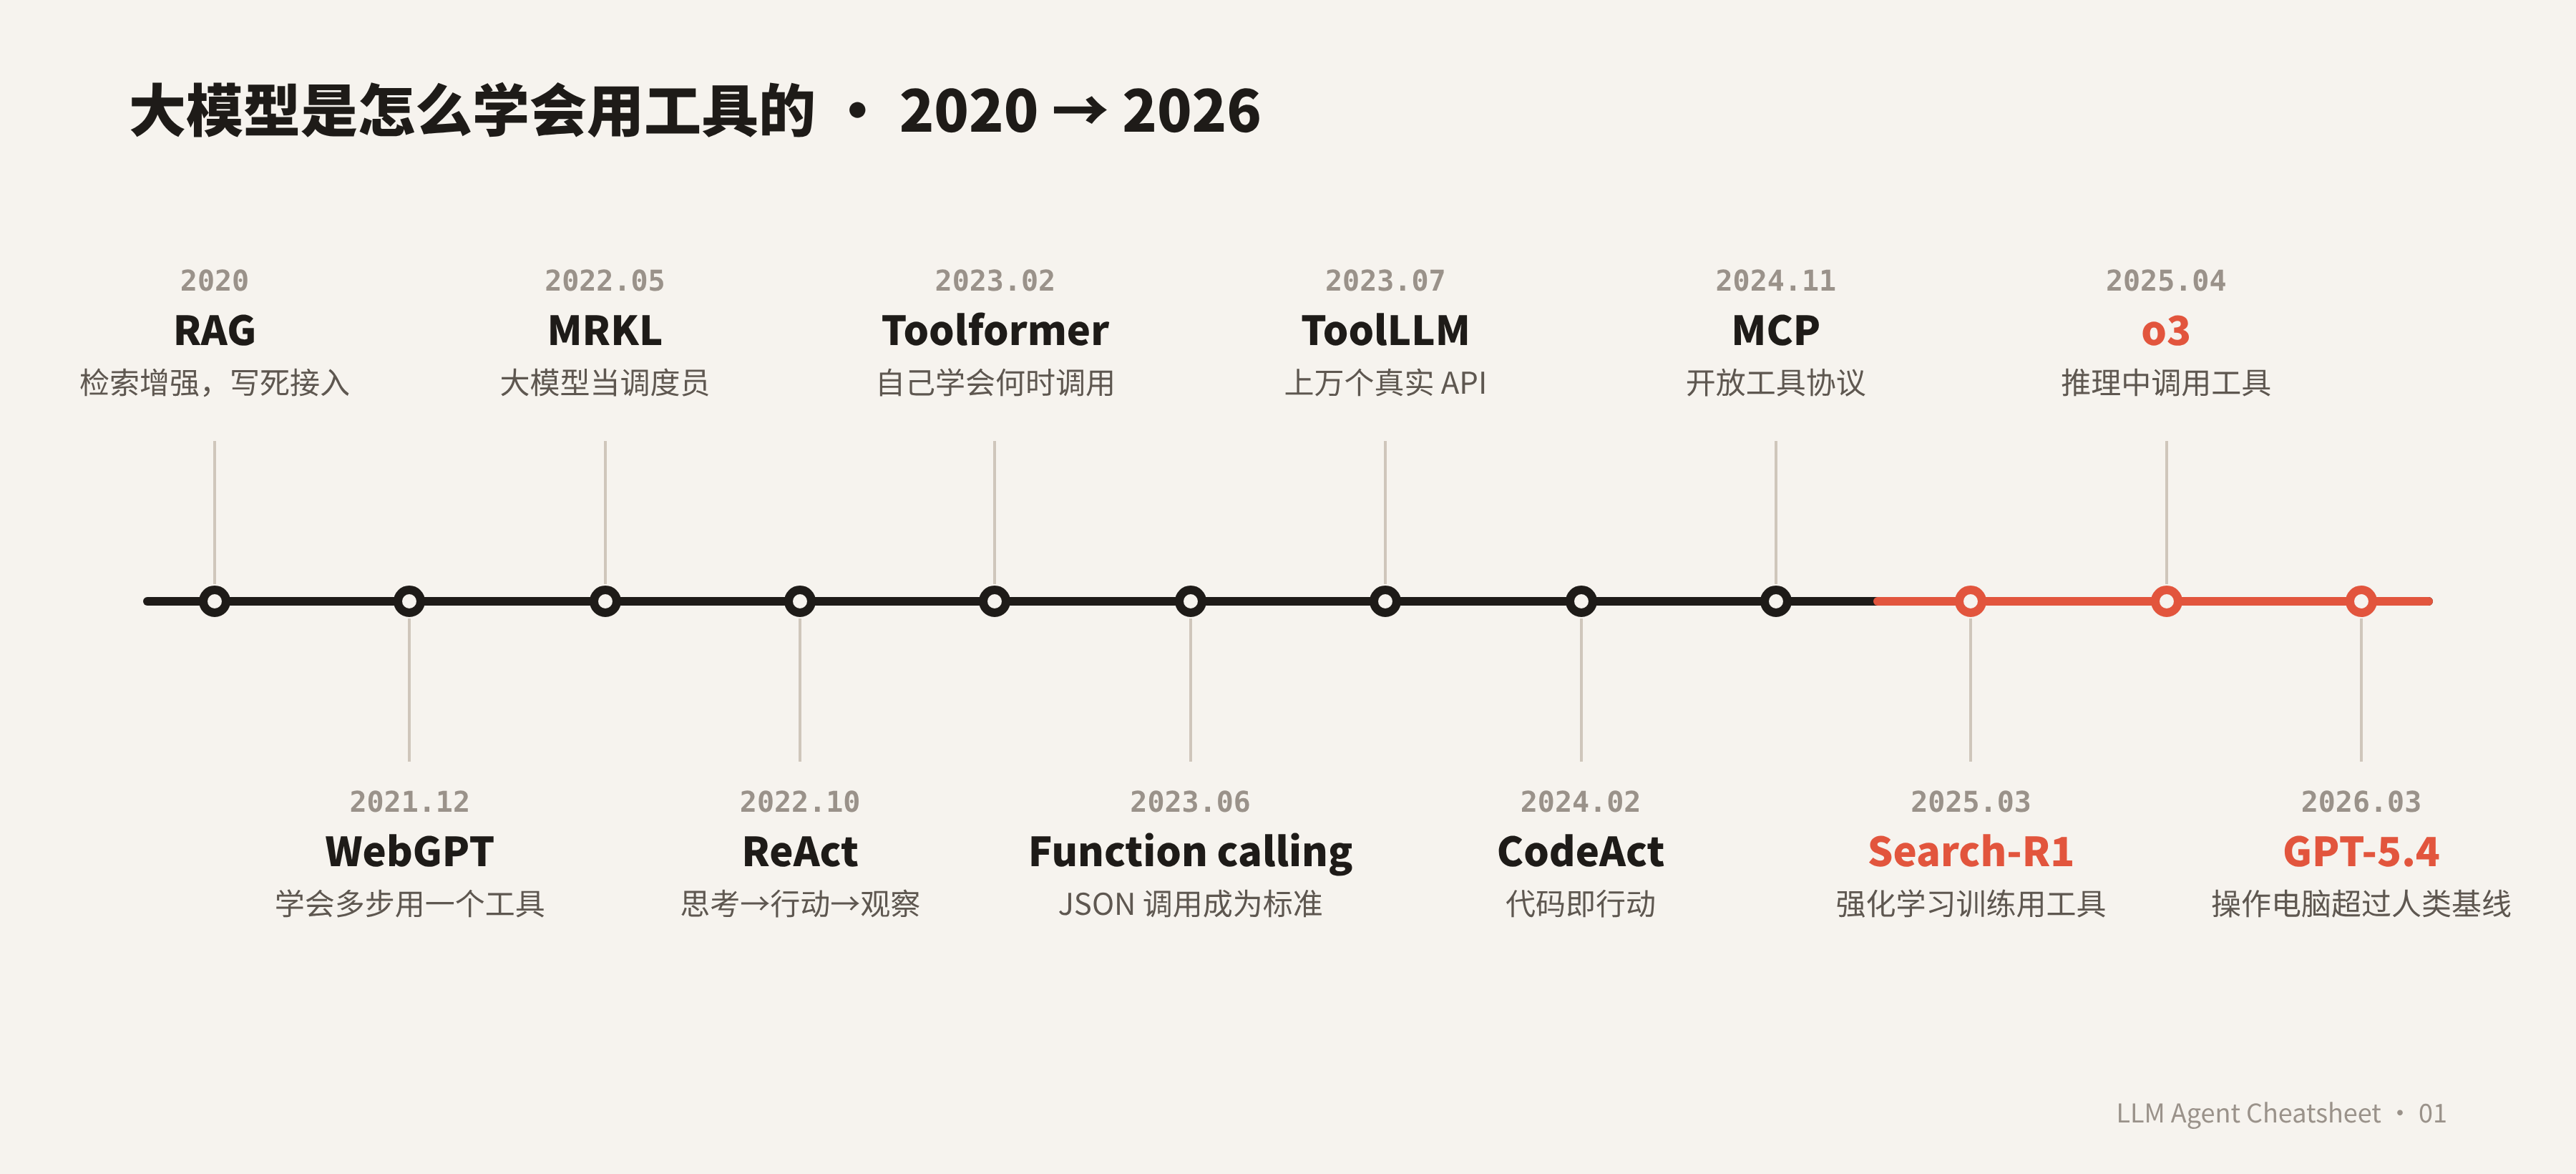
\includegraphics[width=\linewidth]{timeline_zh.png}
\end{tbox}
\end{minipage}\hfill
\begin{minipage}[t]{0.435\linewidth}\vspace{0pt}
\begin{tbox}[title={速查：我的场景该参考哪条线？}]{cpurple}\small
\textbf{精确计算} → 代码解释器：PAL、PoT；RL 版 ToRL、ReTool\\
\textbf{多步检索问答} → ReAct、Self-Ask、IRCoT；RL 版 Search-R1、R1-Searcher\\
\textbf{工具上百上千} → 检索工具文档（Gorilla）、tool search、用代码调 MCP\\
\textbf{长程多轮、要稳定} → CodeAct / ACI 式接口；评测看 τ-bench pass\^{}k、Toolathlon\\
\textbf{有可验证奖励 + 算力} → agentic RL：ToolRL（奖励设计）、ARPO（采样）\\
\textbf{会读不可信内容} → AgentDojo 评测，CaMeL / 设计模式做系统隔离\\[1pt]
{\scriptsize\color{cgray}笔者整理的阅读路由，不是性能排名。}
\end{tbox}
\begin{tbox}[title={入门必读 6 篇（按顺序）}]{cteal}\small
\begin{tabularx}{\linewidth}{@{}l l Y@{}}
1 & \textbf{WebGPT} \ax{2112.09332} & 多步用工具的起点\\
2 & \textbf{ReAct} \ax{2210.03629} & 思考 → 行动 → 观察\\
3 & \textbf{Toolformer} \ax{2302.04761} & 自监督学何时调用\\
4 & \textbf{ToolLLM} \ax{2307.16789} & 上万 API 时问题变成什么\\
5 & \textbf{CodeAct} \ax{2402.01030} & 为什么代码比 JSON 好\\
6 & \textbf{Search-R1} \ax{2503.09516} & 用 RL 训练工具使用\\
\end{tabularx}
\textbf{综述}：Tool Learning with Foundation Models（\ax{2304.08354}）· The Landscape of Agentic RL（\ax{2509.02547}）· Agentic Tool Use in LLMs（\ax{2604.00835}）
\end{tbox}
\end{minipage}

\vspace{2pt}
\begin{minipage}[t]{0.625\linewidth}\vspace{0pt}
\begin{tbox}[title={自测：看完应该能回答（16 问）}]{cpurple}\normalsize\linespread{1.08}\selectfont
\begin{multicols}{2}

\textbf{Q1} RAG-Seq 和 RAG-Tok 的区别？\\
整段答案用同一篇文档 vs 每个 token 可换文档（对文档的边缘化放在乘积外 / 内）。\\[1pt]
\textbf{Q2} Toolformer 的 $L_i^-$ 为什么取“不调用”和“调了不给结果”的较小值？\\
要证明\textbf{结果本身}有用，而不只是调用文本（如问题本身）提供了线索。\\[1pt]
\textbf{Q3} ReAct 比 CoT 好在哪、差在哪？\\
事实性好（CoT 失败 56\% 来自幻觉）；但会陷入重复循环、被无用搜索结果带偏 → 两者组合最好。\\[1pt]
\textbf{Q4} DFSDT 和 ReAct 的关键区别？\\
可以回溯、扩展时参考兄弟节点生成不同动作；ReAct 是单链，一步错就难回头。\\[1pt]
\textbf{Q5} Gorilla 为什么要“检索感知训练”？\\
API 文档会更新；训练时带文档 → 推理时能利用新文档，减少编造参数。但检索差时可能更糟。\\[1pt]
\textbf{Q6} MCP 的 Tools / Resources / Prompts 区别？\\
由谁控制：模型决定调用 / 应用决定附加 / 用户主动选用。\\[1pt]
\textbf{Q7} CodeAct 为什么比 JSON 行动省轮数？\\
一个代码块里就能写循环、条件和变量，组合多个调用；JSON 每轮只能调一次。\\[1pt]
\textbf{Q8} Agentic RL 为什么要 mask 工具返回 token？\\
那些 token 不是模型生成的；计入损失会让模型学“预测工具输出”，梯度有偏、训练不稳。\\[1pt]
\textbf{Q9} pass@$k$ 和 pass\^{}$k$ 各衡量什么？\\
至少一次成功（能力上限）vs $k$ 次全部成功（可靠性）；部署更看后者。\\[1pt]
\textbf{Q10} 为什么提示层防御不够？\\
攻击者可以针对防御自适应优化（The Attacker Moves Second）；需要系统层隔离控制流与数据流（CaMeL）。\\[1pt]
\textbf{Q11} WebGPT 为什么要求回答只基于 Quote？\\
让每个说法都能追溯到原文，人工评估时可以核查事实。\\[1pt]
\textbf{Q12} Self-Ask 的“组合性差距”说明什么？\\
模型会答子问题但不会组合；且不随规模缩小 → 需要显式分解（+ 搜索）。\\[1pt]
\textbf{Q13} LATS 比 ReAct 多了什么、代价是什么？\\
树搜索 + 价值估计 + 反思；需要可回退环境、调用量成倍增加。\\[1pt]
\textbf{Q14} 为什么 2025 年后工具“定义”本身成了瓶颈？\\
几十个 MCP 服务器的 schema 就能占满上下文 → tool search、按需加载、代码调用。\\[1pt]
\textbf{Q15} ReTool 为什么先做冷启动 SFT？\\
让模型先学会“写代码 → 读解释器输出”的格式，RL 才有有效的探索起点。\\[1pt]
\textbf{Q16} “致命三要素”是哪三个？\\
私有数据 + 不可信内容 + 对外通信；三者同时具备就可能被窃取数据。
\end{multicols}
\end{tbox}
\end{minipage}\hfill
\begin{minipage}[t]{0.365\linewidth}\vspace{0pt}
\begin{tbox}[title={关键数字速记}]{cred}\normalsize\renewcommand{\arraystretch}{1.12}
\begin{tabularx}{\linewidth}{@{}l Y@{}}
\toprule
WebGPT & ELI5 偏好：56\% 胜示范者，69\% 胜 Reddit\\
PAL & GSM8K 比 PaLM-540B CoT 高 15 个点\\
ReAct & HotpotQA 35.1 EM（+CoT-SC）；ALFWorld 71 vs 45\\
APIBench & 1,645 个 API\\
ToolBench & 16,464 API / 3,451 工具 / 126,486 条\\
Reflexion & HumanEval 91\% vs GPT-4 80.1\%\\
LATS & HumanEval 92.7\%\\
Voyager & 独特物品 3.3×，里程碑最快 15.3×\\
CodeAct & 成功率最多 +20\%，动作最多 −30\%\\
SWE-agent & SWE-bench 12.5\%，Lite 18.0\%\\
WebArena & GPT-4 14.41\% vs 人类 78.24\%\\
GAIA & GPT-4 + 插件 15\% vs 人类 92\%\\
τ-bench & gpt-4o $<$50\%；零售 pass\^{}8 $<$25\%\\
ToRL & 7B AIME24 43.3\%\\
ReTool & 32B AIME 67\%（400 步）vs 文本 RL 40\%\\
BrowseComp & GPT-4o 1.9\% → Deep Research 51.5\%\\
OSWorld & 38.1 → 61.4 → 75.0\%（人类 72.4\%）\\
Toolathlon & 最好 38.6\%\\
CaMeL & 可证明安全 77\%（无防御 84\%）\\
Code exec + MCP & 150k → 2k token\\
\bottomrule
\end{tabularx}
\end{tbox}
\end{minipage}

\vfill
{\scriptsize\color{cgray}日期为首次公开月份（arXiv v1 或官方发布）；机构为第一作者主要单位；数字取自原文主结果，不同设置下可能不同。完整中英双语版与全部链接：GitHub \texttt{EvenEureka/llm-agent-cheatsheet}。发现错误欢迎指出。}

\end{document}
